\documentclass{article}

% if you need to pass options to natbib, use, e.g.:
% \PassOptionsToPackage{numbers, compress}{natbib}
% before loading nips_2018

% ready for submission
%\usepackage{nips_2018}

% to compile a preprint version, e.g., for submission to arXiv, add
% add the [preprint] option:
\usepackage[]{aistats2019}

% to compile a camera-ready version, add the [final] option, e.g.:
% \usepackage[final]{nips_2018}

% to avoid loading the natbib package, add option nonatbib:
% \usepackage[nonatbib]{nips_2018}

\usepackage[utf8]{inputenc} % allow utf-8 input
\usepackage[T1]{fontenc}    % use 8-bit T1 fonts
\usepackage{hyperref}       % hyperlinks
\usepackage{url}            % simple URL typesetting
\usepackage{booktabs}       % professional-quality tables
\usepackage{amsfonts}       % blackboard math symbols
\usepackage{nicefrac}       % compact symbols for 1/2, etc.
\usepackage{microtype}      % microtypography

\usepackage{amsmath}
\usepackage{graphicx}
\usepackage[normalem]{ulem}
\usepackage{xcolor}

\hypersetup{%
  colorlinks,
  linkcolor={blue!50!black},
  citecolor={blue!50!green!50!black},
  urlcolor={red!50!black}
}

% The \author macro works with any number of authors. There are two
% commands used to separate the names and addresses of multiple
% authors: \And and \AND.
%
% Using \And between authors leaves it to LaTeX to determine where to
% break the lines. Using \AND forces a line break at that point. So,
% if LaTeX puts 3 of 4 authors names on the first line, and the last
% on the second line, try using \AND instead of \And before the third
% author name.

% !TEX root =  nips_dtfa.tex

%% OPTIONAL MACRO DEFINITIONS
% operators
\newcommand{\argmax}{\operatornamewithlimits{argmax}}
\newcommand{\argmin}{\operatornamewithlimits{argmin}}

% fractions, derivatives
\newcommand{\pdff}[2]{\frac{\partial #1}{\partial #2}}
\newcommand{\fdff}[2]{\frac{\delta #1}{\delta #2}}
\newcommand{\ifrac}[2]{#1 \:/\: #2}

% conditional probability 
\newcommand{\p}[2]{\ensuremath{p(#1 \mid #2)}}
\newcommand{\q}[2]{\ensuremath{q(#1 \mid #2)}}
\renewcommand{\d}[1]{\ensuremath{\!\!d#1 \:}}

% vectors
\renewcommand{\vec}[1]{\ensuremath{\boldsymbol{#1}}}
\renewcommand{\v}[1]{\vec{#1}}
\newcommand{\x}{\ensuremath{\v{x}}}
\newcommand{\y}{\ensuremath{\v{y}}}
\newcommand{\z}{\ensuremath{\v{z}}}
\newcommand{\h}{\ensuremath{\v{\eta}}}
\renewcommand{\u}{\ensuremath{u}}
\renewcommand{\q}{\ensuremath{\theta}}
\renewcommand{\l}{\ensuremath{\lambda}}
\renewcommand{\t}{\ensuremath{\tau}}
\newcommand{\f}{\ensuremath{\phi}}

% misc symbols
\newcommand{\KL}[2]{\ensuremath{D_{\rm KL}\left(#1 \:\middle\vert\middle\vert\: #2\right)}}
\renewcommand{\L}{\ensuremath{\mathcal{L}}}
\renewcommand{\P}{\ensuremath{{\mathcal P}}}
\renewcommand{\S}{\ensuremath{\mathcal{S}}}
\renewcommand{\O}{\ensuremath{\mathcal{O}}}
\newcommand{\C}{\ensuremath{\mathcal{C}}}
\newcommand{\Q}{\ensuremath{\mathcal{Q}}}
\newcommand{\V}{\ensuremath{\mathcal{V}}}
\newcommand{\F}{\ensuremath{\mathcal{F}}}
\newcommand{\U}{\ensuremath{\mathcal{U}}}
\newcommand{\E}{\ensuremath{\mathcal{E}}}
\newcommand{\G}{\ensuremath{\mathcal{G}}}
\newcommand{\M}{\ensuremath{\mathcal{M}}}
\newcommand{\N}{\ensuremath{\mathcal{N}}}
\newcommand{\bs}{\backslash}
\newcommand{\td}{\tilde}

\newcommand{\indicator}[2]{\ensuremath{\mathbb{I}{[{#1}={#2}]}}}
\newcommand*{\dom}{\ensuremath{\mathrm{dom}}}



\newcommand{\scf}{\textsc{f}}
\newcommand{\scg}{\textsc{g}}
\newcommand{\scw}{\textsc{w}}
\newcommand{\scp}{\textsc{p}}
\newcommand{\scs}{\textsc{s}}
\newcommand{\scx}{\textsc{x}}

\begin{document}

\twocolumn[

\aistatstitle{Modeling Individual Differences in fMRI Data\\ with Neural Topographic Factor Analysis}

\aistatsauthor{ Anonymous }

\aistatsaddress{ Anonymous }

\aistatsauthor{ Anonymous }

\aistatsaddress{ Anonymous } ]

% \aistatsauthor{ Eli Sennesh \And Zulqarnain Khan \And Jennifer Dy }

% \aistatsaddress{ Northeastern University \And Northeastern University \And Northeastern University }

% \aistatsauthor{ J. Benjamin Hutchinson \And Ajay Satpute \And Jan-Willem van de Meent }

% \aistatsaddress{ University of Oregon \And Northeastern University \And Northeastern University } ]


\begin{abstract}
Contemporary neuroimaging studies produce a large volume of data (Gigabytes) for a small number of participants (20-50). This poses major challenges in studies where we would like to reason about individual variation in the response of participants to a particular stimulus.
%and when we want to discover full-brain networks using functional connectivity matrices which normally scale with number of voxels (generally around 50,000 voxels). 
To address these challenges, we propose deep topographic factor analysis, a new family of models for the analysis of functional neuroimaging data that combine the computational scalability of matrix factorization with variational Bayesian methods for reasoning about the distribution of neural responses in studies with small sample sizes. 
\end{abstract}

\section{Introduction}

Analysis of neuroimaging studies is both a big data problem and a small data problem. A scan of a single participant typically involves 10s of stimuli, each comprising 100s of time points at 10,000s of spatial locations (often referred to as voxels). Because of this, statistical methods need to scale to gigabytes of data. At the same time, reasoning about the variation in neural response across participants is a small data problem, since a typical study considers a cohort of 20-50 participants. 

In this paper we introduce Neural Topographic Factor Analysis (NTFA), a family of models for analysis of fMRI data that is geared towards reasoning about individual variations across small numbers of individuals and stimule. NTFA extends existing techniques based on factor analysis to incorporate embeddings for subjects and stimuli. 

[FINISH INTRO]

\section{Topographic Factor Analysis}

%  While there are different existing approaches to reduce the size of the data by reducing the number of voxels, these generally use functionally (\cite{craddock2012whole} \cite{gonzalez2015tracking} \cite{power2011functional} \cite{thomas2011organization}) or anatomically (\cite{betzel2017modular}\cite{fox2010clinical} \cite{shen2013groupwise}) defined voxels clusters or regions of interest (ROIs), in summary these approaches try to utilize the intuition about how the brain works, this can range from pre-selecting a small number of ROIs to reduce the $V\text{x}V$ connectivity matrix to $V\text{x}V_{ROI}$ matrix, to examining full brain connectivity patterns via ROI-to-ROI connectivity matrices.[24]  
 
 Factor analysis methods have recently gained traction in the analysis of neuroimaging data. These models decompose fMRI measurements $Y \in \mathbb{R}^{T\text{x}V}$ into a product $Y \simeq W F$ between lower-rank matrices of weights $W \in \mathbb{R}^{T\text{x}K}$ and factors $F \in \mathbb{R}^{K\text{x}V}$, where, typically $K<<V$. Representing many voxels and timepoints in terms of a much smaller set of spatio-temporal factors greatly reduces the dimensionality of the original data, while at the same time capturing meaningful regularities. Examples of factor analysis methods that have been applied to fMRI data include Principal Component Analysis (PCA) \cite{abdi2010principal}, Independent Component Analysis (ICA) \cite{hyvarinen2001independent}, Hyper-Alignment (HA) \cite{haxby2011common}, Topographic Latent Source Analysis (TLSA) [18]. %and Topographic Factor Analysis (TFA) \cite{manning2014topographic}, among others. TFA and its Hierarchical extension \cite{manning2014hierarchical} is what we build our method on and therefore we will discuss this in more detail in the next section




%\jwm{ToDo write a couple more sentences here.} \jbh{if it's true, I'd definitely highlight how such embeddings could be learned from the data (completely data-driven) or constrained by psychological variables (e.g. responses to a fear questionnaire) by an experimenter, thus enabling an explicit choice (precise specification) over the confirmatory/exploratory nature of the analysis while making minimal assumptions about the structure of the neural data per se}
%\as{JW: "extend" seems like a weak word. Can we amp it up? Also, I added in "functional runs" below}
%\subsection{Topographic Factor Analysis}

The methods that we will propose here will build on topographic factor analysis (TFA) \cite{manning2014topographic} and Hierarchical Topographic Factor Analysis \cite{htfa} (HTFA). %,  which we will generalize and extend to incorporate a notion of participant and subject embeddings using neural networks.
TFA is a probabilistic factor analysis model that uses radial basis functions to define spatially smooth factors. Each factor is parameterized in terms of a spatial mean and a width, which are treated as latent variables in a probabilistic model. 
%They then use the principles of Bayesian inference to reason about probable locations for each factor given a set of fMRI measurements. 
Concretely, suppose that we were to consider a series of $N$ measurements (i.e. functional runs) each of which contain $T$ time points for voxels at $V$ spatial positions. TFA approximates each measurement $Y_{n} \simeq W_{n} F_{n}$ as a product between a matrix of $K$ time-varying weights $W_n \in \mathbb{R}^{T \times K}$ and a matrix $F_n \in \mathbb{R}^{K \times V}$ of $K$ spatially-varying factors. TFA assumes a hierarchical Gaussian prior over weights
\begin{align*}
	W_{n,t,k}
    &\sim 
    \mathcal{N}(\mu^\scw_{n,k}, \sigma^\scw_{n,k}),
    &
	\mu^\scw_{n,k}
   	&\sim 
    p(\mu^\scw),
    &
	\sigma^\scw_{n,k} 
   	&\sim 
    p(\sigma^\scw).
\end{align*}
To ensure spatial smoothness of factor values $F_{n,k,v}$ at similar voxel positions $x^\scg_v \in \mathbb{R}^3$, TFA defines each factor in terms of a kernel function $\kappa$. This kernel function is normally a radial basis function (RBF), which models each factor as a Gaussian peak at a spatial location $x_{n,k}^\scf \in \mathbb{R}^3$, whose width is determined by the kernel hyper-parameters $\rho^\scf_{n,k}$, 
\begin{align}
	\label{eq:tfa-factor-kernel}
	F_{n,k,v}
    &= 
    \kappa(x^\scg_v, x^\scf_{n,k} \,;\, \rho^\scf_{n,k})
    .
\end{align}
TFA assumes Gaussian priors over both the spatial positions and widths, 
\begin{align}
	x^\scf_{n,k} 
    &\sim 
    p(x^\scf),
    &   
	\rho^\scf_{n,k} 
    &\sim 
    p(\rho^\scf).
\end{align}
The advantage of assigning a probabilistic interpretation to factor analysis is that we can incorporate additional assumptions in order to capture variation and similarities between multiple sets of measurements. HTFA \cite{manning2014hierarchical}, introduces variables $\bar{x}^\scf_k$ and $\bar{\rho}^\scf_k$ that represent the mean spatial positions and widths for each factor across measurements, 
\begin{align} 
    x^\scf_{n,k} 
    &\sim 
    p(x^\scf_{n,k} \mid \bar{x}^\scf_{k})
    ,
    &
    \bar{x}^\scf_{k} 
    &\sim
    p(\bar{x}^\scf)
    ,
    \\
    \rho^\scf_{n,k} 
    &\sim 
    p(\rho^\scf_{n,k} \mid \bar{\rho}^\scf_{k})
    ,
    &
    \bar{\rho}^\scf_{k} 
    &\sim
    p(\bar{\rho}^\scf).
\end{align}
This prior is able to model individual variation to an extent, in the sense that factor positions and widths for individual measurements are allowed to vary relative to a shared mean. However, the hierarchical Gaussian prior in HTFA is primarily geared towards characterizing the average response across measurements. 

\begin{figure*}[!t]
    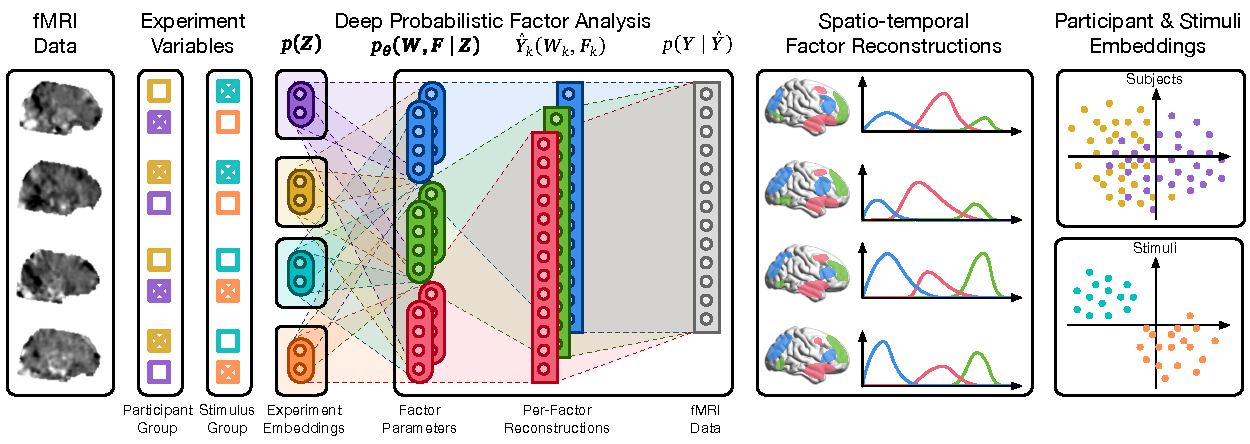
\includegraphics[width=\textwidth]{figures/deep-tfa.pdf}
    \caption{\label{fig:subject-embedding} Overview of Neural Topographic Factor Analysis (NTFA). We extend topographic factor analysis (TFA) \cite{manning2014topographic,manning2014hierarchical} to decompose the fMRI signal into distinct factors (shown in red, green and blue in the figure) that correspond to spatially and temporally related brain activity across individuals. We model subjective experience by representing using embedding vectors to represent subjects (yellow and purple) and stimuli (cyan and orange), which together define the distribution on the factor parameters for each measurement.}
\end{figure*}


\section{Neural Topographic Factor Analysis}
\label{sec:dtfa-basic}

In NTFA we assume the same likelihood model as TFA, which is to say that we model the fMRI signal as a linear combination of time-dependent weights and spatially varying Gaussian factors. However, rather than assuming a shared prior, NTFA represents individuals and stimuli using \emph{embedding vectors} that characterize the extent to which an individual participant or stimulus deviates from the mean. We then learn a mapping from embeddings to the parameters of the likelihood model, which can be a linear function, or more generally a neural network. This replaces the hierarchical Gaussian prior in HTFA with a (simple) deep generative model.

Concretely, we define participant embeddings $\{z^\scp_1, \ldots, z^\scp_P\}$ and stimulus embeddings $\{z^\scs_1, \ldots, z^\scs_S\}$. For simplicity, we will assume that both embeddings have the same dimensionality, and are distributed according to a Gaussian prior
\begin{align}
    z_{p,d}^\scp &\sim \mathcal{N}(0,1), 
    &
    z_{s,d}^\scs &\sim \mathcal{N}(0,1),
    &
    d = 1, \ldots, D.
\end{align}

For each combination of participant $p$ and stimulus $s$, we define the RBF center $x_{p,s}^\scf$ and width $\rho_{p,s}^\scp$ in terms of a neural mapping 
\begin{align}
    x_{p,s}^\scf &\leftarrow \bar{x}^\scf + \eta^{x}_\theta \left( \eta^h_\theta (z_p^\scp, z_s^\scs) \right),
    &    
    \bar{x}^\scf \sim p(\bar{x}^\scf),
    \\
    \rho_{p,s}^\scf &\leftarrow \bar{\rho}^\scf + \eta^{\rho}_\theta \left( \eta^h_\theta (z_{p}^\scp, z_{s}^\scs) \right),
    &    
    \bar{\rho}^\scf \sim p(\bar{\rho}^\scf).
\end{align}
Here $\eta_\theta^h$, $\eta_\theta^x$, and $\eta_\theta^\rho$, are simple neural networks, each parameterized by some set of weights $\theta$, which model the individual variation relative to mean parameters $\bar{x}^\scf$ and $\bar{\rho}^\scf$ shared across participants and stimuli. 

% \begin{align}
%     x^T &\sim \mathcal{N}(\theta_{x}) \\
%     \rho^T &\sim \mathcal{N}(\theta_{\rho}) \\
%     \Delta x &\leftarrow \eta^{\sc{X}} \left( \eta^h (z^\scp, z^\scs) \right) \\
%     \Delta \rho &\leftarrow \eta^\rho \left( \eta^h (z^\scp, z^\scs) \right) \\
%     x, \rho &\leftarrow x^T + \Delta x, \rho^T + \Delta \rho
% \end{align}
To define the distribution on $W_{p,s}$, we similarly use a network $\eta^\scw$ to model individual variation,
\begin{align}
    \mu_{p,s}^\scw, \sigma_{p,s}^\scw &\leftarrow \eta^\scw_\theta(\eta^h_\theta(z_p^\scp, z_s^\scs)).
\end{align}
For each time point $t$, we then define the distribution on weights and voxel activations as
\begin{align}
    W_{p,s,t} &\sim \mathcal{N}(\mu_{p,s}^\scw, \sigma_{p,s}^\scw),
    \\
    F_{p,s,k} &\gets \kappa(x^\scf_{p,s,k}, \rho^\scf_{p,s,k}),
    \\
    \hat{Y}_{p,s,t} &\gets W_{p,s,t} \cdot F_{p,s},
    \\
    Y_{p,s,t} &\sim \mathcal{N}\big( \hat{Y}_{p,s,t}, \sigma^\textsc{y}\big).
\end{align}
This generative model defines a posterior distribution $p(W,\bar{x}^\scf,\bar{\rho}^\scf,z^\scp,z^\scs \mid Y)$, which we approximate with a variational distribution $q(W,\bar{x}^\scf,\bar{\rho}^\scf,z^\scp,z^\scs \mid \lambda)$. We jointly optimize the variational parameters $\lambda$ and the network weights $\theta$ by maximizing the lower bound
\begin{align*}
    \mathcal{L}(\theta, \lambda)
    = 
    \mathbb{E}_\lambda
    \left[
    \log 
    \frac{p(Y, W,\bar{x}^\scf,\bar{\rho}^\scf,z^\scp,z^\scs)}
         {q(W,\bar{x}^\scf,\bar{\rho}^\scf,z^\scp,z^\scs \mid \lambda)}
    \right]
    \le 
    \log p_\theta(Y).
\end{align*}


% To train this model, we approximate the posterior  $q_{\lambda_n}(o, z^\scp_n, z^\scs_n, x^T, \rho^T, \Delta W_t) \simeq p_\theta(o, z^\scp_n, z^\scs_n, x^T, \rho^T, \Delta W_t \mid Y_n)$ by maximizing the evidence lower bound with respect to the generative parameters $\theta$ and the variational parameters $\lambda$,
% \begin{align}
% 	\mathcal{L}(\theta, \lambda) 
%     &= 
%     \sum_{n=1}^N
%     \mathbb{E}_{q_{\lambda_n}(z^\scw_n, z^\scf_n)}
%     \left[
%     \log
%     \frac{p_\theta(Y_n, z^\scw_n, z^\scf_n)}
%          {q_{\lambda_n}(z^\scw_n, z^\scf_n)}
%     \right]
%     \le 
%     \sum_{n=1}^N \log p(Y_n)
%     .
% \end{align}
To optimize this objective, we use Probabilistic Torch, a library for deep generative models that extends the PyTorch deep learning framework  \cite{narayanaswamy2017learning,2018probtorch}. This makes it comparatively straightforward to optimize objectives such as the evidence lower bound for general classes of user-defined models. 
%As a proof of concept, we have implemented the basic NTFA variant that we describe in this section and trained it on the Pie Man dataset \cite{simony2016dynamic}, which has also in the past been used evaluate TFA. In Figure~\ref{fig:pieman}, we show the mean weight embeddings and the factor embeddings, which while preliminary, show a reasonable degree of separation for measurements in which subjects are either at rest, or listening to the audio of a story. 

\begin{figure}[!t]
    \begin{center}
    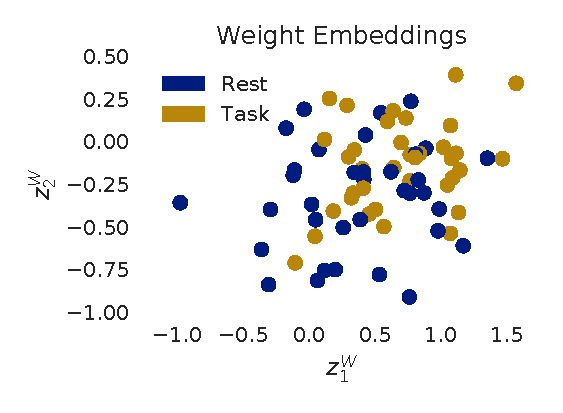
\includegraphics[width=2.5in]{figures/embedding_z_w_rest_intact.pdf}
    \hspace{4ex}
    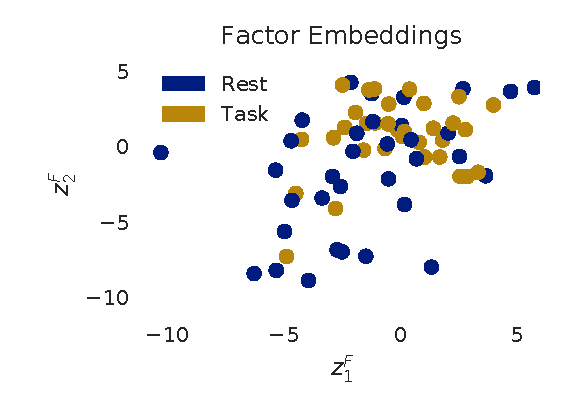
\includegraphics[width=2.5in]{figures/embedding_z_f_rest_intact.pdf}
    \end{center}
    \vspace{-15pt}
    \caption{\label{fig:pieman} Preliminary results from NTFA analysis of the Pie Man Dataset \cite{simony2016dynamic}. Each dot represents a single measurement in which a subject is either at rest, or is listening to Pie Man (a story from the Moth \cite{pieman}).}
%(\emph{Left}) Time-averaged weight embeddings $\bar{z}^\scw_{n} = \frac{1}{T} \sum_{t=1}^T z^\scw_{n,t}$ (\emph{Right}) Factor embeddings $z^\scf_n$.}
\end{figure}


More generally, the advantage of incorporating neural networks into the generative model is that it enables us to both capture average effects and explicitly reason about individual variation. The parameters $\theta^\scw$ and $\theta^\scf$ are shared across all measurements $n$, allowing us to capture statistical regularities within an experiment. At the same time, the use of neural networks ensures that differences in embeddings can be mapped onto a wider range of variation in spatial and temporal responses. For example, the  hierarchical Gaussian priors in HTFA implicitly assume that variations are uncorrelated for different factors $k$, whereas neural networks allow us to capture such correlations by jointly predicting all $K$ factors from a single embedding. 

While neural networks in general can have thousands or even millions of parameters, we emphasize that the parametrization in NTFA can in fact have in a \emph{lower} number of trainable parameters than the one in TFA and HTFA. The reason for this is that TFA and HTFA assume fully factorized variational distributions for which the number of parameters scales as $O(N T K)$. In NTFA, the networks $\eta^\scw$ and $\eta^h$ will have $O(DK)$ and $O(EK)$ parameters respectively, whereas the variational distribution will have $O(N T D + N E)$ parameters, which in general means that we can obtain a lower-dimensional parametrization by choosing embedding dimensions $D$ and $E$ that are smaller than the number of factors $K$. 
 

\section{Experiments}

We base our experiments partly on experiments conducted by Manning et al. in their latest iteration of HTFA \cite{}. We utilize 3 datasets, two publicly available datasets, and one dataset collected in-house. A short description of each dataset follows: 

\begin{itemize}
    
    \item \textbf{Synthetic Data}: To demonstrate how NTFA works, we created a synthetic fMRI dataset. The dataset consists of 2 groups of 10 subjects each, with Group 1 doing a hypothetical set of similar tasks (for example watching videos) and Group 2 doing a different set of tasks (for example listening to audio) . The data is generated by first generating the participant embeddings $\{z_1^P,...,z_{20}^P \}$ and stimulus embeddings $\{ z_1^S,...,z_{20}^S\}$, and generating factors and weights as functions of these embeddings in such a way that for Group 1, the voxels in front right region of the brain have higher activations, while for Group 2 voxels in the Back Left region have higher activations. 

    \item \textbf{Pieman Dataset} \cite{}: Participants listen to an audio recording of a story; 36 particpants listen to an intact version of the story, 18 participants listen to time-scrambled recordings of the same story where paragraphs were scrambled, 25 particpants listen to word-scrambled version and 36 particpants lay in rest condition.
    
    \item \textbf{Sherlock Dataset} \cite{}: 17 participants viewin an episdoe from BBC television show Sherlock. For each participant the full dataset comprises of 43,371 voxels over 1976 TRs.
    
    \item \textbf{Sherlock Merlin Dataset}: \cite{} 18 Participants watch Sherlock Movie and listen to the audio recording of Merlin Movie, while 18 other participants watch Merlin Movie and listen to the audio of Sherlock Movie. 
    
    \item \textbf{AffVids Dataset} \cite{}: An in-house dataset where various participants are subjected to stimuli with normative fear ratings of spider, heights, and social situations in addition to resting state data. We also have self reports from participants rating these stimuli. 
\end{itemize}

Following \cite{HTFA} on Pieman and Sherlock Datasets, we measure the decoding accuracy based on Voxels, Nodes, Inter-Subject Functional Connectivity (ISFC) \cite{HTFA32} and a 50-50 mix of Node and ISFC,   using the same number of factors for HTFA and for NTFA. The computation of each of these decoding accuracies is outlined here, for more detail please refer to \cite{HTFA}:

\begin{itemize}
    \item \textbf{Voxel Based Decoding Accuracy}: Randomly divide participants for each stimulus into two groups. For each stimulus compute the mean voxel activities within a sliding window, For each group of participants compare the resulting set of $\mathbb{R}^V$ vectors using Pearson Correlations. Then the first group's time windows are labelled using the second group's time windows with which they are highly correlated. The proportion of correctly labelled time windows is called voxel based decoding accuracy. This effictively is a measure of whether there's some usable information in the raw data or not.
    
    \item \textbf{Node Based Decoding Accuracy}: The same procedure as Voxel Based Decoding Accuracy is repeated accept this time instead of raw data, the Weight Matrix from NTFA and HTFA is used.
    
    \item \textbf{ISFC Based Decoding Accuracy}: This measures correlations between brain regions of different individuals in each of the above mentioned sliding windows, the decoding accuracy drived from this is a measure of stimulus-driven activity \cite{HTFA}.
    
    \item \textbf{Mixed Decoding Accuracy}: This is a 50-50 mix of Node Based and ISFC Based Decoding Accuracy, since they capture different sources of activity \cite{HTFA}
    
\end{itemize}


\bibliographystyle{plain}
\bibliography{aistats_dtfa.bib} 

\end{document}
